\chapter{Experiments}


\comEA{Add the new estimators. Is it methodology? Because it is still an example.}
\section{Assessing exact and approximate samplers}
A central distinction in this chapter is between asymptotic exactness and finite-time computational efficiency. 
An MCMC transition kernel may be $\pi$-invariant, and hence exact in the usual Markov chain sense, while still being practically inefficient if its accept-reject mechanism is driven by rare events or high-variance unbiased estimators. 
For this reason, we do not compare methods only at a fixed number of iterations. 

Instead, we report the computational time required to reach a target effective sample size for $\eta$, together with distributional discrepancies from a reference posterior. 
Since $\eta$ is one-dimensional, we use the empirical Wasserstein distance as the primary convergence diagnostic. 
KL and Jensen-Shannon divergences are reported only as secondary diagnostics, since they require density estimation.

For exact Poisson and Bernoulli-factory constructions, we additionally monitor the local envelope parameter $\lambda$, the realized Poisson count $K$, the variability of $\log \widehat I$, invalid factors, and, for DCBF, recursive agreement attempts. 
These diagnostics separate correctness of the invariant distribution from practical viability of the resulting algorithm.


\subsection{Building an estimator}

The most simple approach is the harmonic estimator, since

\begin{equation*}
    c_0(\eta) = \bE_{\theta\sim\pi_0}\qty[L_0(\theta\mid D_0)^\eta].
\end{equation*}

Then, we define $\delta_a$ as

\begin{equation}
    \delta_a(\eta, \theta_1, \dots, \theta_K) = \dfrac{1}{K} \sum_{i=1}^K L_0(\theta_i\mid D_0)^\eta
\end{equation}

And with this estimator we can then employ a Portkey Barker's~\cite{vats2021} to sample from the power posterior. 

This $\delta_a$ has a major two-sided feature, while it is easy to sample from the initial prior, its efficiency is low due to its large non-informativeness.

In order to improve the efficiency, we can produce an importance sampling estimator by concentrating the probability density around the $\hat{\theta}_{\text{MLE}}$, which gives us

\begin{equation*}
c_0(\eta) = \int_{\theta\in\Theta} L_0(\theta\mid D_0)^\eta \pi_0(\theta)\dd{\theta} = \bE_{\theta\sim\pi_{\text{MLE}}}\qty[L_0(\theta\mid D_0)^\eta\dfrac{\pi_0(\theta)}{\pi_{\text{MLE}}(\theta)}].    
\end{equation*}


We can then define $\delta_b$ as:

\begin{equation}
    \delta_b(\eta, \theta_1, \dots, \theta_K) = \dfrac{1}{K} \sum_{i=1}^K L_0(\theta_i\mid D_0)^\eta\dfrac{\pi_0(\theta_i)}{\pi_{\text{MLE}}(\theta_i)}.
\end{equation}

\comEA{Different compatibility scenarios.}

\subsection{The choice of $\lambda$ and $c$ for the Gaussian likelihood with known $\Sigma$.}

Considering the functional form of our estimator $\widehat{\Delta}(\eta, \eta') = (\eta' - \eta) \log L_0\qty(D_0\mid\widetilde{\theta})$ and that $L_0$ is the likelihood of $D_0 = \{d_{01}, \dots, d_{0N}\}$ where each $d_{0j} \sim \cN_d(\theta, \Sigma)$ for $j = 1, \dots, N$ with known $\Sigma$, we can find that 

$$\argmax_{\theta \in \Theta} \log L_0\qty(D_0\mid\theta) = \hat{\theta}_{\text{MLE}}= \dfrac{1}{N}\sum_{j=1}^N d_{0j},$$

and, therefore, we have that

$$\max_{\theta \in \Theta} \log L_0\qty(D_0\mid\theta) = -\frac{N d}{2}\log(2\pi) - \frac{N}{2}\log\det\Sigma - \frac{N}{2}\operatorname{tr}(\Sigma^{-1}S),$$

 where $S= \frac{1}{N}\sum_{j=1}^N(x_j - \hat{\theta}_{\text{MLE}})(x_j - \hat{\theta}_{\text{MLE}})^\top$


 
\subsection{The choice of $\lambda$ and $c$ for the exponential family}

\comEA{Produce analytical results for exponential family. I have it somewhere.}

A canonical exponential family has the following density: 

\begin{equation}
    L(X\mid \theta) = b(X) \exp{\theta^\top t(X) - c(\theta)},\, \theta \in \Theta \subseteq \bR^d,
\end{equation}

where $\Theta$ is open and connected.

\section{Using Exact Methods as Baseline}
\comEA{Here I'd like to use the best exact method to assess the quality of the approximate methods}

\section{Numeric Experiments}


\subsection{Convergence to the baseline}

We evaluate the proposed estimators under a multivariate Gaussian model with known covariance ($p = 3$, $\Sigma = I_3$, $\Sigma_0 = 2I_3$), placing weakly informative Beta$(1,1)$ priors on $\eta$ and an initial $\cN_3(0, \Sigma_0)$ prior on $\theta$.
Historical and current datasets each contain $N_0 = N = 50$ observations.
Three discrepancy scenarios are constructed by shifting the historical data mean by $\delta \in \{0.1, 0.5, 1.0\}$ per coordinate, representing low, moderate, and high conflict between historical and current information.

Rather than running each method for a fixed number of iterations, we adopt a convergence-based protocol: each estimator is run in independent batches of four chains and 5\,000 iterations until the two-sample Kolmogorov--Smirnov (KS) distance between its accumulated posterior draws for $\eta$ and the Stan HMC baseline drops below 0.05.
The number of chains and total wall-clock time required to reach this threshold serve as our primary efficiency metrics.
The exact algorithm---which uses the closed-form normalising constant ratio---acts as a reference.
We compare it against three approximate pseudo-marginal methods: the prior-importance estimator ($\delta_a$), the MLE importance-sampling estimator ($\delta_b$), and the power-posterior estimator.


\begin{figure}[H]
    \centering
    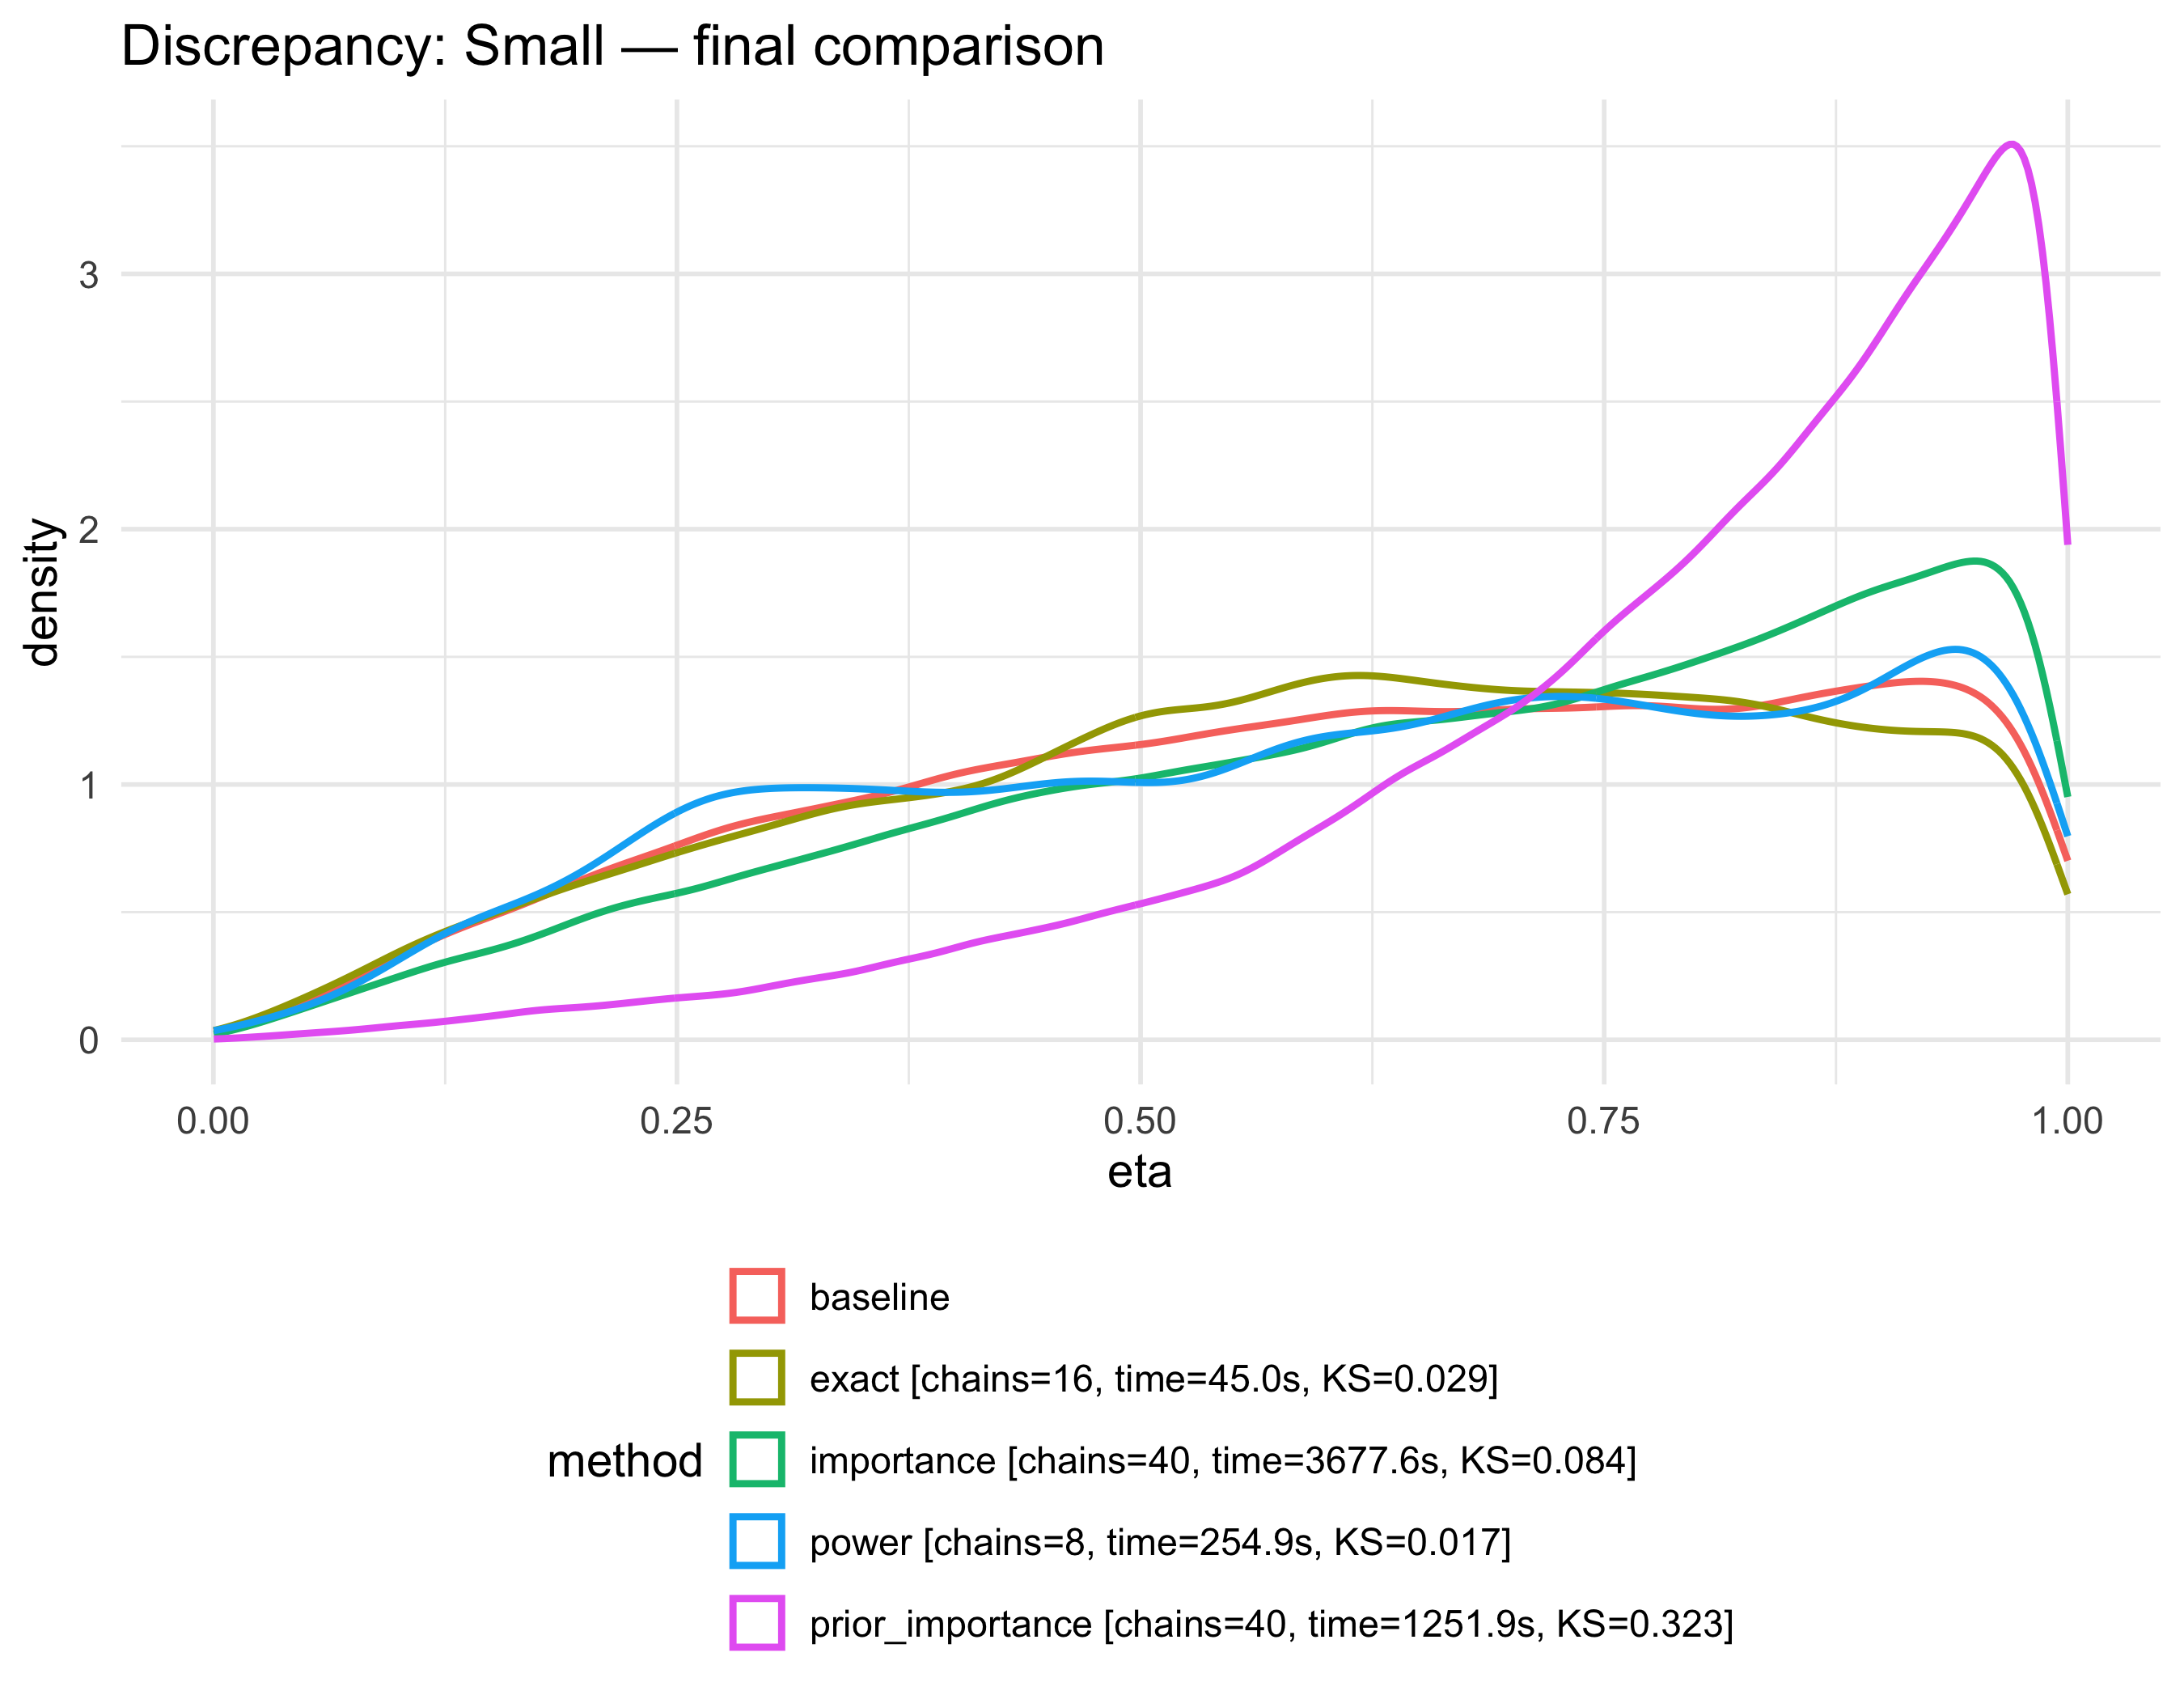
\includegraphics[width=\linewidth]{figures/ch5/convergence_small.png}
    \caption{Posterior densities for $\eta$ under low discrepancy ($\delta = 0.1$). Each approximate estimator label reports the total number of chains run, wall-clock time, and final KS distance to the Stan baseline.}
    \label{fig:convergence-small}
\end{figure}

\begin{figure}[H]
    \centering
    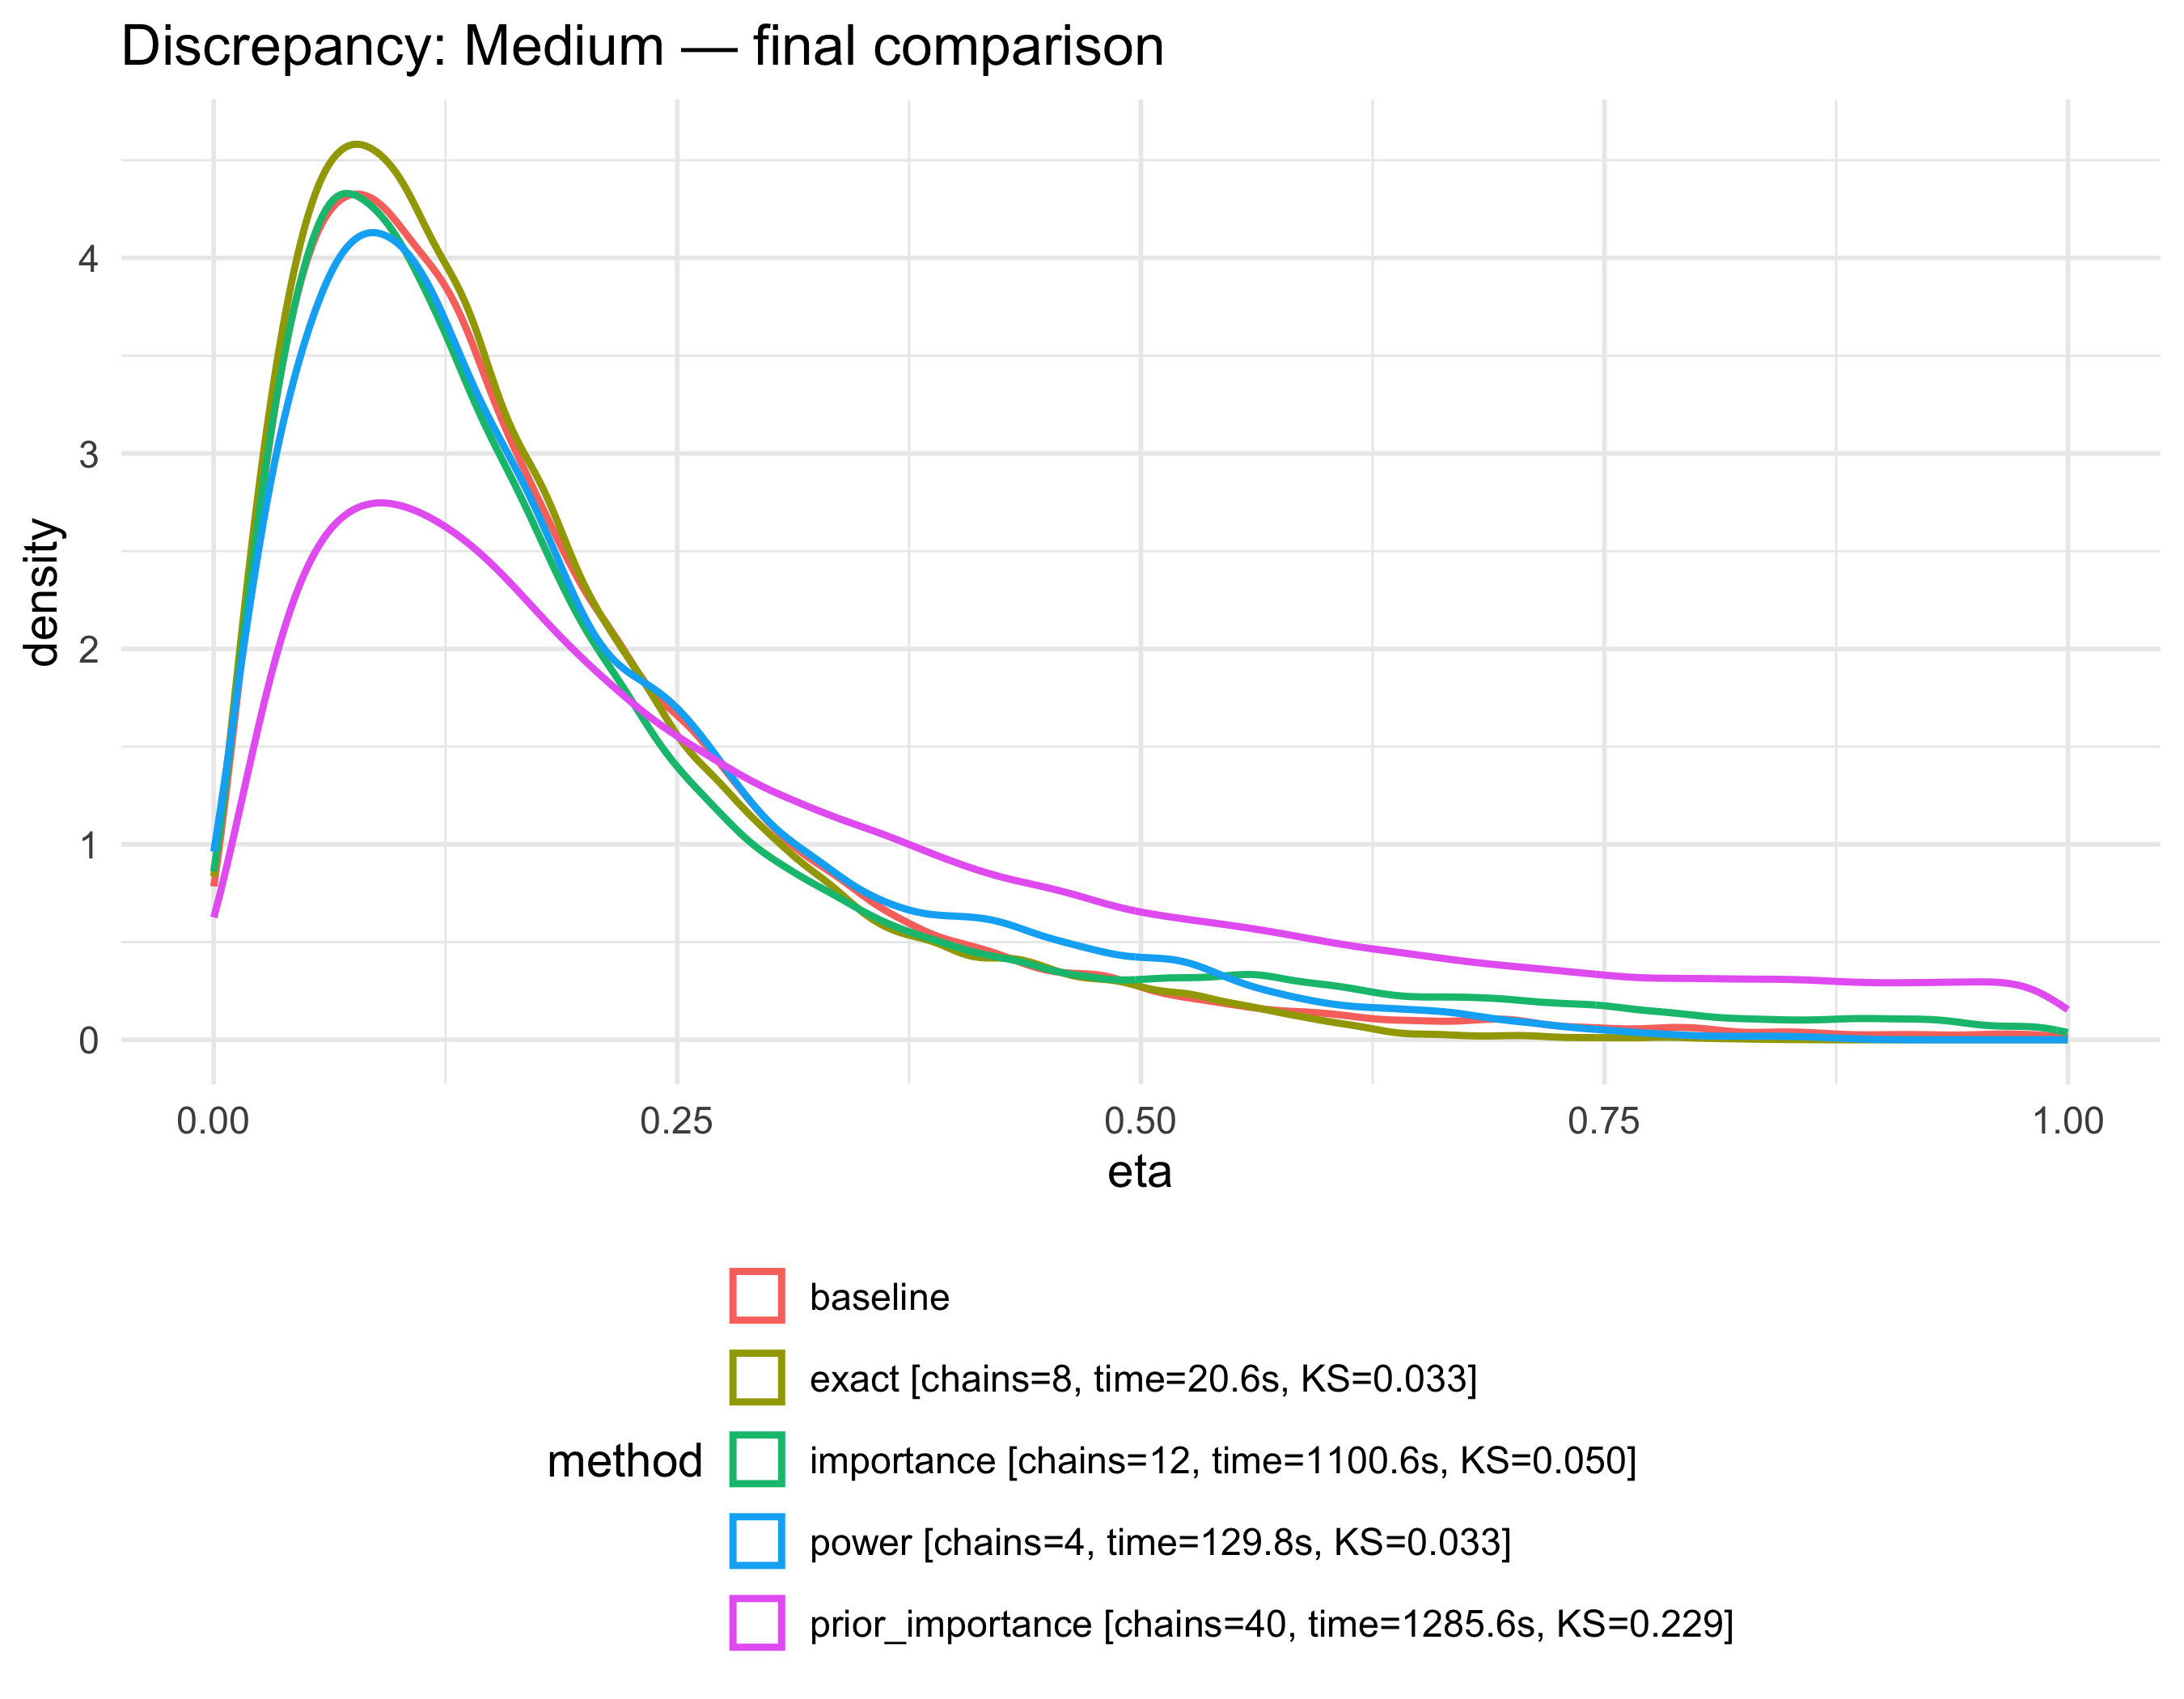
\includegraphics[width=\linewidth]{figures/ch5/convergence_medium.png}
    \caption{Posterior densities for $\eta$ under moderate discrepancy ($\delta = 0.5$).}
    \label{fig:convergence-medium}
\end{figure}

\begin{figure}[H]
    \centering
    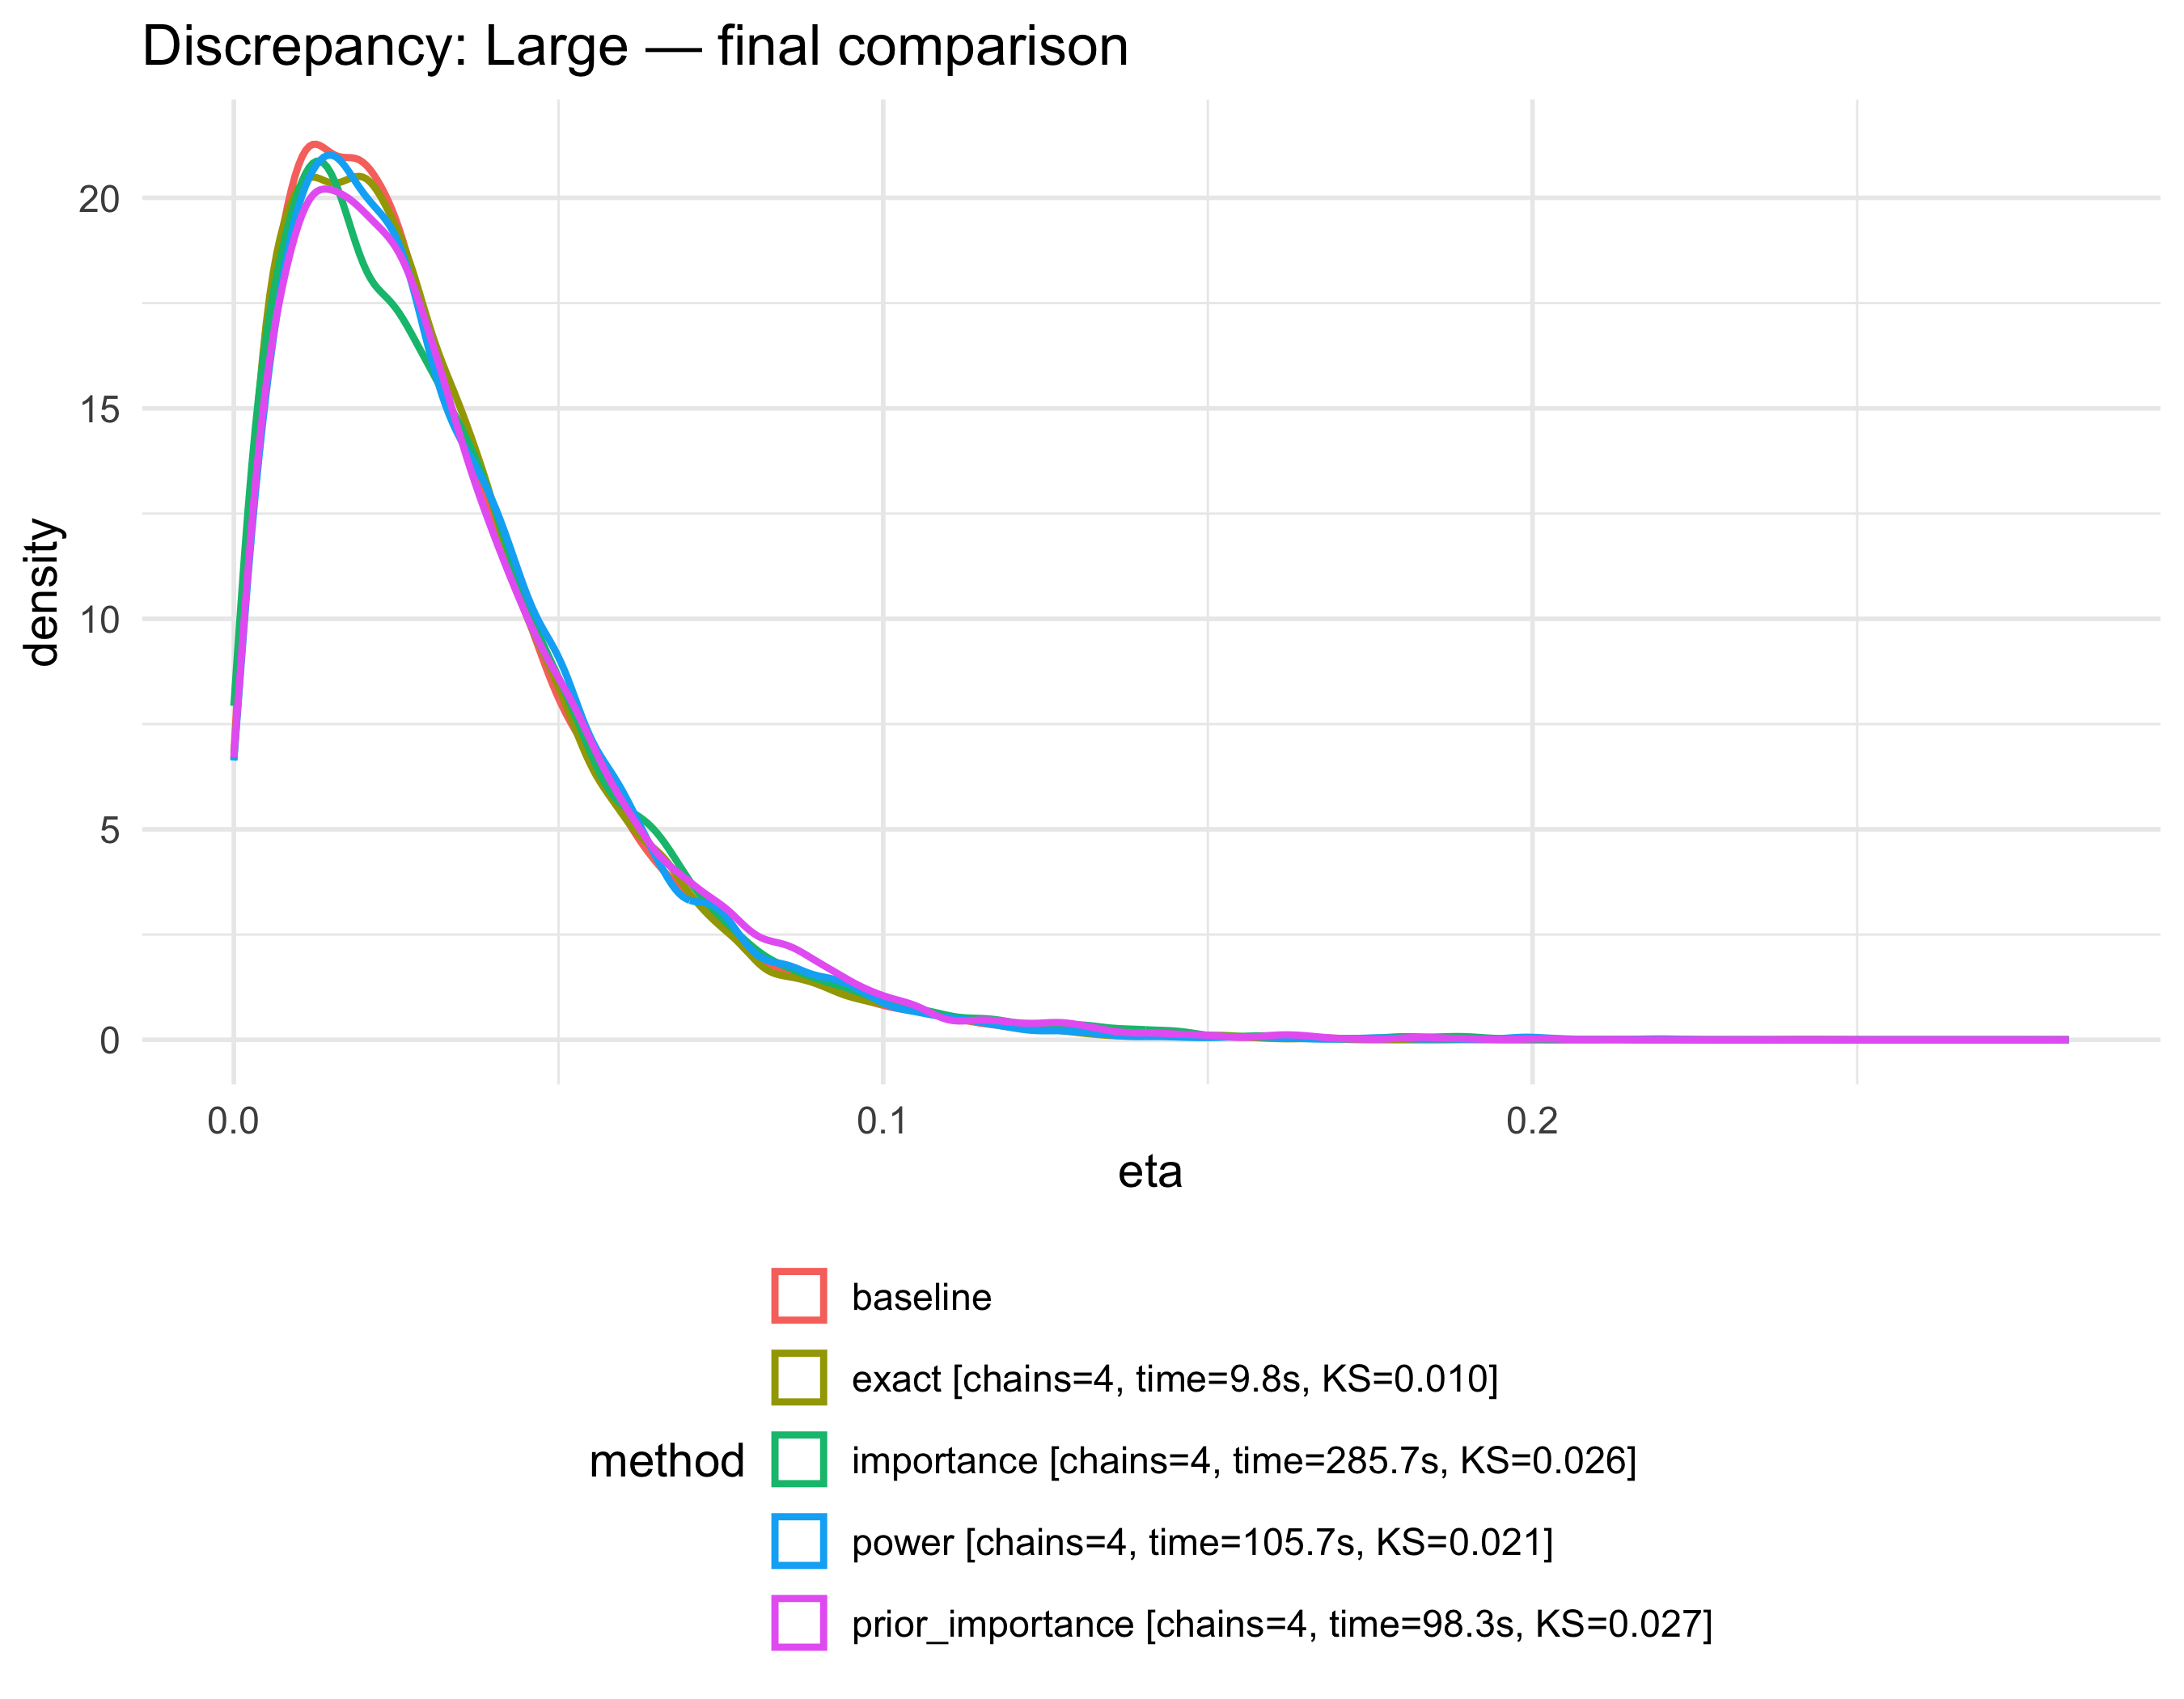
\includegraphics[width=\linewidth]{figures/ch5/convergence_large.png}
    \caption{Posterior densities for $\eta$ under high discrepancy ($\delta = 1.0$). Under strong conflict between datasets the posterior concentrates near zero and all methods converge in a single batch.}
    \label{fig:convergence-large}
\end{figure}

\begin{table}[ht]
    \centering
    \begin{tabular}{lcccccc}
    \hline
    & \multicolumn{2}{c}{Small ($\delta=0.1$)} & \multicolumn{2}{c}{Medium ($\delta=0.5$)} & \multicolumn{2}{c}{Large ($\delta=1.0$)} \\
    Method & Chains & KS & Chains & KS & Chains & KS \\
    \hline
    Exact             &  16 & 0.029 &  8 & 0.033 & 4 & 0.010 \\
    Prior-importance  &  40 & 0.323 & 40 & 0.229 & 4 & 0.027 \\
    Importance        &  40 & 0.084 & 12 & 0.050 & 4 & 0.026 \\
    Power             &   8 & 0.017 &  4 & 0.033 & 4 & 0.021 \\
    \hline
    \end{tabular}
    \caption{Total chains required and final KS distance to the Stan HMC baseline. A dash indicates the method reached 10 batches (40 chains) without satisfying the convergence criterion.}
    \label{tab:convergence-comparison}
\end{table}

\subsection{Discussion of results}

The results reveal a consistent pattern across discrepancy regimes.
Under low discrepancy (Figure~\ref{fig:convergence-small}), the posterior for $\eta$ spreads across a wide range, reflecting genuine uncertainty about how much weight to assign to the historical data.
In this regime the estimators differ most sharply: the power estimator converges in just two batches (8 chains, KS$=0.017$), the exact algorithm requires four batches (16 chains, KS$=0.029$), whereas the importance estimator exhausts all ten batches without reaching the threshold (KS$=0.084$) and the prior-importance estimator deviates substantially from the baseline (KS$=0.323$).
The inefficiency of $\delta_a$ here is expected: when the posterior for $\eta$ is diffuse, prior samples for $\theta$ are a poor proposal for the normalising-constant integral, yielding high-variance estimates of the log-ratio.

Under moderate discrepancy (Figure~\ref{fig:convergence-medium}), the posterior shifts toward smaller values of $\eta$, indicating the model has begun to down-weight the historical data.
The power estimator again converges in a single batch (4 chains), the exact algorithm in two, and the importance estimator in three.
The prior-importance estimator still fails to reach the threshold, though its KS distance has improved relative to the low-discrepancy case.

When the two datasets are in strong conflict (Figure~\ref{fig:convergence-large}), the posterior concentrates sharply near $\eta \approx 0$.
In this regime all four estimators converge in a single batch of four chains, and the KS distances are uniformly small.
The sharp concentration of the posterior makes the normalising-constant ratio easy to estimate regardless of the proposal, erasing the differences observed at lower discrepancy levels.

Overall, the power estimator is the most efficient of the three approximate methods: it matches or beats the exact algorithm in chains required across all scenarios.
The prior-importance estimator is consistently the weakest, particularly when the posterior is diffuse.
These findings suggest that the choice of estimator matters most in low-discrepancy settings, where the posterior for $\eta$ is broad and the normalising constant must be estimated accurately over a wide range of values.

\subsection{Linear regression with Normal-Inverse-Gamma priors}
\label{subsec:nig-lm-experiment}

We next consider a Gaussian linear regression model with unknown variance.
This experiment is designed to evaluate the exchange update in a setting where the normalized power prior remains analytically tractable, but the normalizing constant is no longer a simple linear function of the power parameter.
Let $D_0 = (\bfX_0,\bfy_0)$ denote the historical data and let $D = (\bfX,\bfy)$ denote the current data.
We assume
\begin{equation}
    \bfy_0 = \bfX_0 \bfbt + \bfeps_0,
    \qquad
    \bfy = \bfX \bfbt + \bfeps,
\end{equation}
where $\bfeps_0 \sim \cN(\bfzero,\sg \bfI_{n_0})$ and $\bfeps \sim \cN(\bfzero,\sg \bfI_n)$.
The variance $\sg$ is unknown.
The initial prior is Normal-Inverse-Gamma,
\begin{equation}
    \bfbt \mid \sg \sim \cN(\bfmu_0,\sg \bfV_0),
    \qquad
    \sg \sim \InvGam(a,b).
\end{equation}
For a fixed value of $\eta$, the powered prior is given by
\begin{equation}
    \pi_{\eta}(\bfbt,\sg \mid D_0)
    =
    \frac{
        L(D_0 \mid \bfbt,\sg)^\eta \pi_0(\bfbt,\sg)
    }{
        c_0(\eta)
    }.
\end{equation}
The normalizing constant is
\begin{equation}
    c_0(\eta)
    =
    \int_0^\infty
    \int_{\bR^p}
    L(D_0 \mid \bfu,v)^\eta
    \pi_0(\bfu,v)
    \dd \bfu
    \dd v.
\end{equation}
In this model, $c_0(\eta)$ is available in closed form by conjugacy.
This allows us to construct an analytic reference chain for $\eta$ and to validate algorithms that do not directly evaluate $c_0(\eta)$.
The marginal posterior density of $\eta$ is proportional to
\begin{equation}
    \pi(\eta \mid D_0,D)
    \propto
    \frac{
        \pi_A(\eta)
        \Gamma(n/2+\nu_0)
        \abs{\Lambda_0}^{1/2}
        H_0(\eta)^{\nu_0}
    }{
        \abs{\Lambda}^{1/2}
        \Gamma(\nu_0)
        H(\eta)^{\nu_0+n/2}
    }.
    \label{eq:nig-lm-eta-marginal}
\end{equation}
The quantities $\nu_0$, $\Lambda_0$, $H_0(\eta)$, $\Lambda$, and $H(\eta)$ are defined in Appendix~\ref{example:nig_lm}.
Although the analytic expression is available here, the exchange algorithm does not require evaluating $c_0(\eta)$.
Given the current state $(\bfbt,\sg,\eta)$, we propose $\eta'$ and draw an auxiliary value
\begin{equation}
    ({\bfbt}^\star,{\sg}^\star)
    \sim
    \pi_{\eta'}(\bfbt,\sg \mid D_0).
\end{equation}
The exchange log-ratio for the $\eta$ update is
\begin{align}
    \log R_{\mathrm{ex}}
    &=
    (\eta'-\eta)
    \log L(D_0 \mid \bfbt,\sg)
    +
    (\eta-\eta')
    \log L(D_0 \mid {\bfbt}^\star,{\sg}^\star)
    \nonumber
    \\
    &\quad
    +
    \log \frac{\pi_A(\eta')}{\pi_A(\eta)}
    +
    \log \frac{q(\eta \mid \eta')}{q(\eta' \mid \eta)}.
    \label{eq:nig-lm-exchange-log-ratio}
\end{align}
The proposal is then accepted with probability $\min\{1,\exp(\log R_{\mathrm{ex}})\}$.
When the auxiliary draw from $\pi_{\eta'}(\bfbt,\sg \mid D_0)$ is exact, this update has the correct invariant distribution for the normalized power prior.
This follows from the exchange algorithm for doubly-intractable distributions, where an auxiliary draw from the proposed normalized model cancels the unknown ratio of normalizing constants in the Metropolis-Hastings acceptance probability~\cite{murray2012}. 
The exchange algorithm therefore provides an exact update for $\eta$ under the powered-prior simulation assumption.
This assumption is satisfied in the present experiment because the powered prior is Normal-Inverse-Gamma.

We compare three methods.
The first method is an analytic Metropolis-Hastings reference that evaluates Equation~\eqref{eq:nig-lm-eta-marginal}.
The second method is the exchange Metropolis-Hastings update in Equation~\eqref{eq:nig-lm-exchange-log-ratio}.
The third method is a path-sampling pseudo-marginal method based on a Monte Carlo approximation of the normalizing constant ratio.
The path-sampling method is included as a computational baseline and is classified according to the exactness of the estimator used in its acceptance ratio.
If the estimator is not non-negative and unbiased for the required marginal target, the method is treated as approximate rather than exact.
This distinction follows the pseudo-marginal principle, where exactness requires a non-negative unbiased estimator of the target density on an extended space~\cite{andrieu2009}.

We generate three discrepancy scenarios between the historical and current regression coefficients.
In the small-discrepancy scenario, the current coefficient vector is close to the historical coefficient vector.
In the medium-discrepancy scenario, the current coefficient vector is moderately shifted.
In the large-discrepancy scenario, the current coefficient vector is substantially shifted.
The expected qualitative behavior is that the posterior distribution of $\eta$ moves toward smaller values as the discrepancy increases.
This reflects reduced borrowing from the historical data when the historical and current data-generating mechanisms are less compatible.

The main diagnostic is the one-dimensional Wasserstein distance from each method to the analytic reference.
We report this distance separately for $\eta$, $\norm{\bfbt}_2$, and $\sg$.
We also report posterior means, posterior standard deviations, effective sample sizes, acceptance rates, and runtime.
The norm $\norm{\bfbt}_2$ summarizes the magnitude of the regression coefficient vector, while $\sg$ is reported separately because it represents the residual variance and should not be combined with $\bfbt$ into a single geometric average.

\begin{figure}[ht]
    \centering
    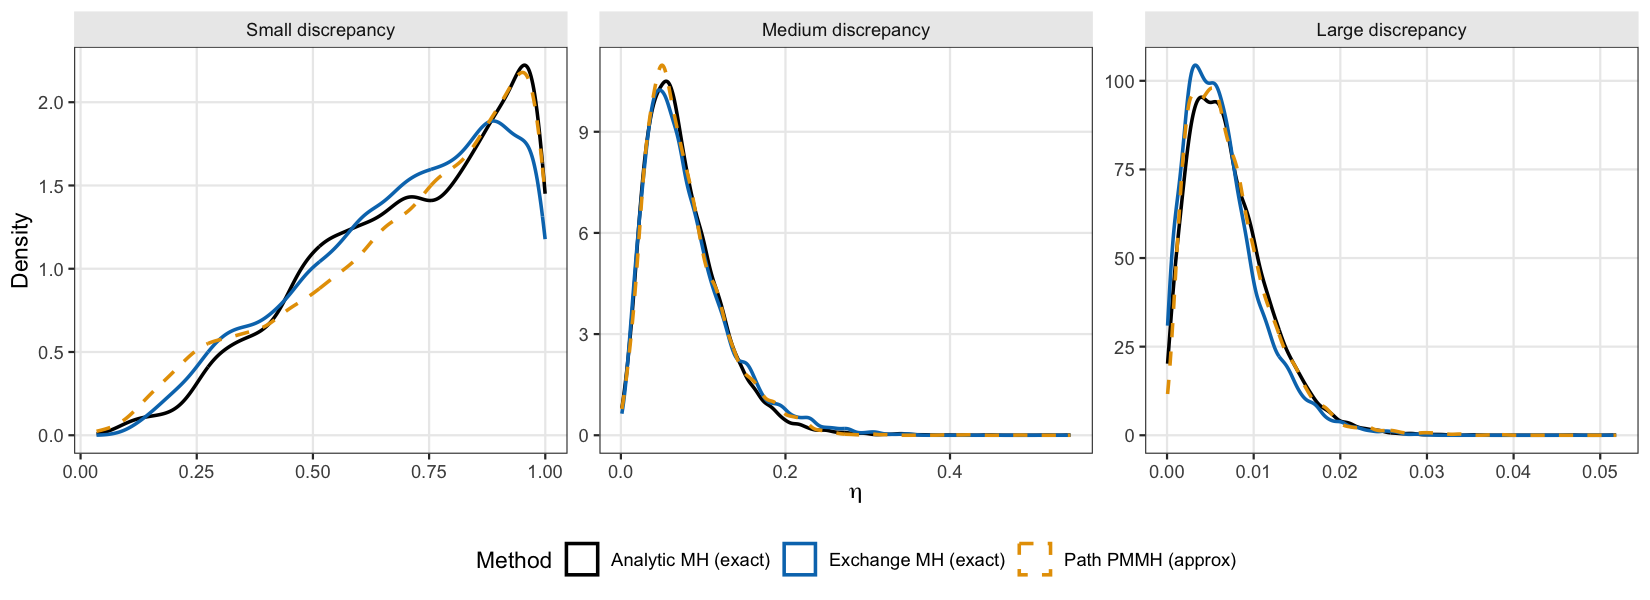
\includegraphics[width=\textwidth]{../software/experiments/results/nig_lm_exchange/posterior_eta_all_discrepancies.png}
    \caption{Posterior density of $\eta$ for the linear regression NPP experiment across discrepancy scenarios.}
    \label{fig:nig-lm-eta-density}
\end{figure}

\begin{figure}[ht]
    \centering
    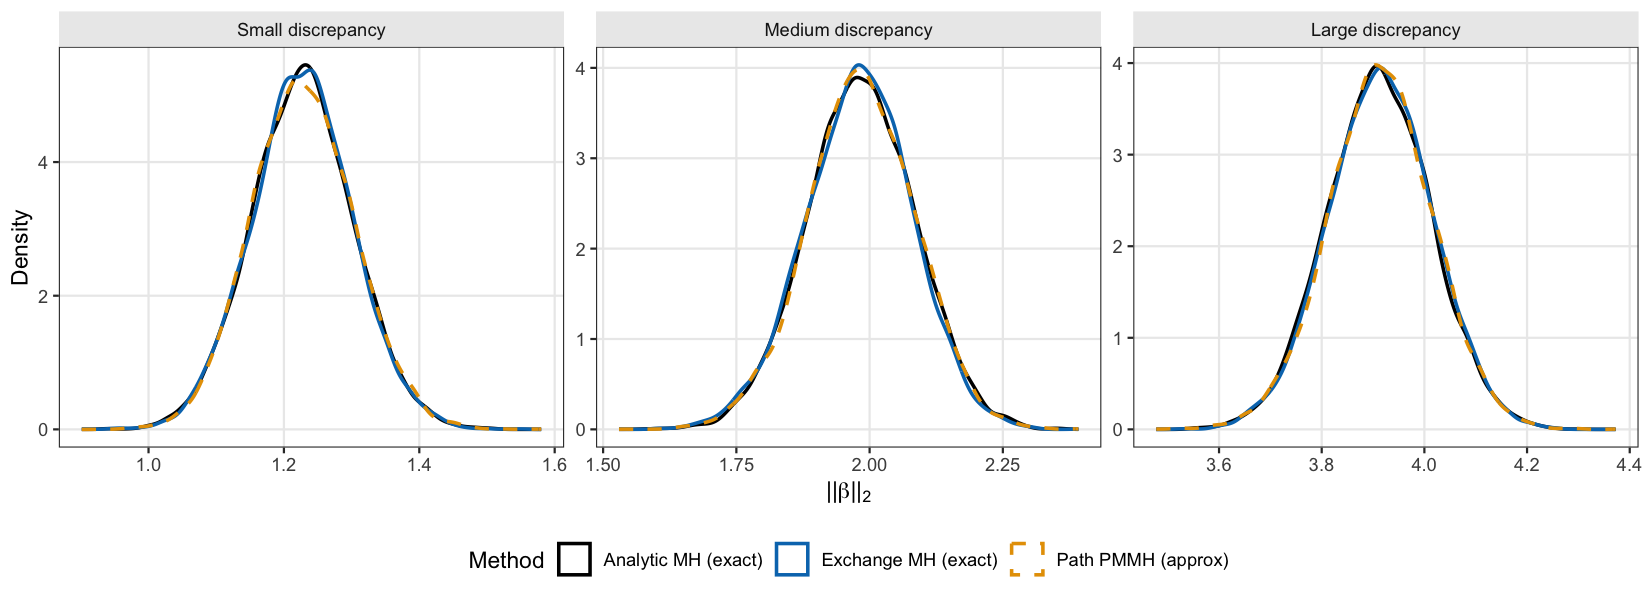
\includegraphics[width=\textwidth]{../software/experiments/results/nig_lm_exchange/posterior_beta_norm_all_discrepancies.png}
    \caption{Posterior density of $\norm{\bfbt}_2$ for the linear regression NPP experiment across discrepancy scenarios.}
    \label{fig:nig-lm-beta-norm-density}
\end{figure}

\begin{figure}[ht]
    \centering
    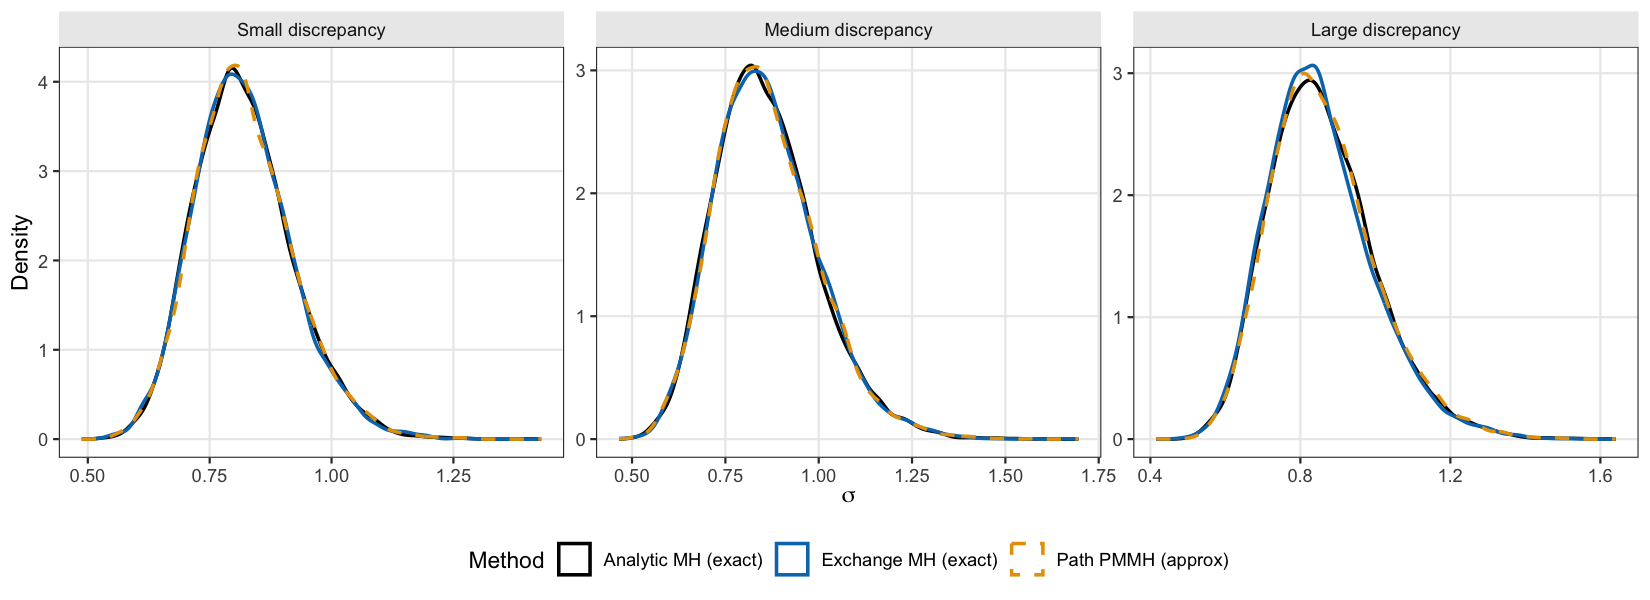
\includegraphics[width=\textwidth]{../software/experiments/results/nig_lm_exchange/posterior_sigma_all_discrepancies.png}
    \caption{Posterior density of $\sg$ for the linear regression NPP experiment across discrepancy scenarios.}
    \label{fig:nig-lm-sigma-density}
\end{figure}

\begin{table}[ht]
  \centering
  \begin{tabular}{llcccccc}
  \hline
  Scenario & Method & $W_\eta$ & $W_{\|\beta\|}$ & $W_\sigma$ & ESS$_\eta$ & Acc.\ $\eta$ & Time (s) \\
  \hline
  Small & Analytic MH & 0.000 & 0.000 & 0.000 & 195 & 0.928 & 3.1 \\
  Small & Exchange MH & 0.019 & 0.001 & 0.002 & 222 & 0.902 & 1.6 \\
  Small & Path PMMH & 0.022 & 0.001 & 0.001 & 199 & 0.913 & 31.6 \\
  \hline
  Moderate & Analytic MH & 0.000 & 0.000 & 0.000 & 717 & 0.859 & 3.2 \\
  Moderate & Exchange MH & 0.003 & 0.003 & 0.002 & 557 & 0.797 & 1.6 \\
  Moderate & Path PMMH & 0.002 & 0.001 & 0.002 & 797 & 0.837 & 32.5 \\
  \hline
  Large & Analytic MH & 0.000 & 0.000 & 0.000 & 682 & 0.863 & 3.1 \\
  Large & Exchange MH & 0.001 & 0.003 & 0.009 & 577 & 0.824 & 1.6 \\
  Large & Path PMMH & 0.000 & 0.003 & 0.003 & 694 & 0.858 & 32.1 \\
  \hline
  \end{tabular}
  \caption{Diagnostic comparison for the linear regression NPP experiment with Normal-Inverse-Gamma priors. Wasserstein distances are computed against the analytic MH baseline within each discrepancy scenario.}
  \label{tab:nig-lm-exchange-diagnostics}
\end{table}


\begin{table}[ht]
  \centering
  \begin{tabular}{llcccccc}
  \hline
  Scenario & Method & $\bar{\eta}$ & $\mathrm{sd}(\eta)$ & $\overline{\|\beta\|}$ & $\mathrm{sd}(\|\beta\|)$ & $\bar{\sigma}$ & $\mathrm{sd}(\sigma)$ \\
  \hline
  Small & Analytic MH & 0.697 & 0.208 & 1.227 & 0.076 & 0.820 & 0.101 \\
  Small & Exchange MH & 0.679 & 0.217 & 1.228 & 0.075 & 0.818 & 0.101 \\
  Small & Path PMMH & 0.705 & 0.227 & 1.229 & 0.075 & 0.821 & 0.101 \\
  \hline
  Medium & Analytic MH & 0.077 & 0.049 & 1.984 & 0.102 & 0.862 & 0.137 \\
  Medium & Exchange MH & 0.080 & 0.051 & 1.981 & 0.101 & 0.863 & 0.137 \\
  Medium & Path PMMH & 0.078 & 0.047 & 1.983 & 0.102 & 0.863 & 0.138 \\
  \hline
  Large & Analytic MH & 0.007 & 0.005 & 3.912 & 0.102 & 0.863 & 0.142 \\
  Large & Exchange MH & 0.007 & 0.005 & 3.915 & 0.101 & 0.854 & 0.140 \\
  Large & Path PMMH & 0.007 & 0.005 & 3.915 & 0.103 & 0.860 & 0.141 \\
  \hline
  \end{tabular}
  \caption{Posterior summaries for the NIG linear regression NPP experiment.}
  \label{tab:nig-lm-exchange-summaries}
\end{table}
